In order to provide an overall schema of the whole architectural structure of our application, it seems relevant to show the mappings of the main components in such a high-level representation. \\
At the top of the structure there is the client tier, the layer which allows the direct interation with users. This layer is composed by the user interfaces of the mobile application and the web pages of the web application. \\
The core of the architecture consists in the business tier, the layer in charge of providing the computations to assolve the functional requirements and to make them available through the presentation tier for the users. The main components of this tier are the Entity Java Beans of the application server and the servlets and Java Server Pages/Faces of the web server. \\
At the bottom of the architectural structure there is the persistence level, which essentially consists in a database. The database stores all the data available and manages to answer the queries made by the components of the business tier to retrieve information useful for computational processess.\\ 



\begin{figure} 
\begin{center}

\makebox[\textwidth]{%
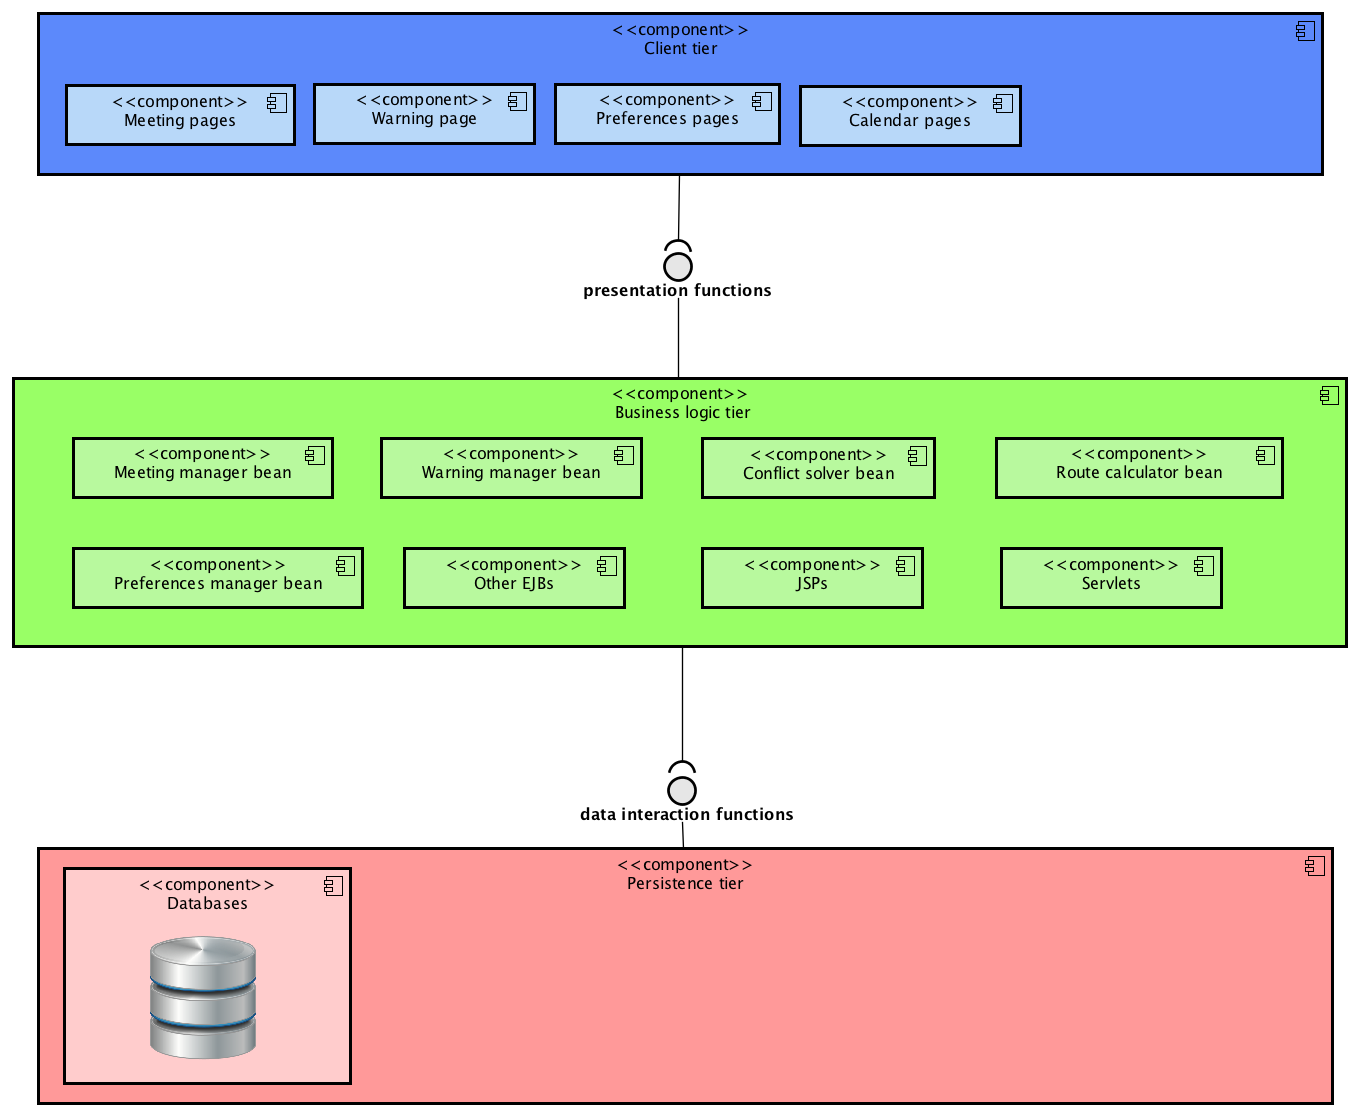
\includegraphics[width=1.5\linewidth]{images/HLcomponentdiagram} 
}
\caption{High-level component diagram} 
\label{fig:hlcomponentdiagram} 


\end{center}
\end{figure} 
